
\section{Architecture}
\label{sec:architecture}

The distributed and decentralized \textsc{c}ollabo\textsc{rat}ive
\textsc{e}ditor \CRATE developed in web languages only: HTML, CSS, and mostly
JavaScript. It comprises four layers:
\begin{enumerate}[(i)]
\item the graphical user interface that renders the document to the users
  (cf. Figure~\ref{img:screenshot}). Each local update is immediatly applied to
  the document view for real-time sake. Then, the update is applied to the
  replicated data type;
\item the replicated data type layer that represents the local document
  (cf. §\ref{sec:structure}). It is in charge of providing the metadata
  necessary to order each character identically anywhere;
\item the causality layer that tracks semantic causality between operations,
  e.g., the removal of a character cannot precede its insertion.
\item the network layer that
  \begin{inparaenum}
  \item builds a network of browsers for each editing session and
  \item uses it to propagate the updates to all collaborators
    (cf. §\ref{sec:network});
  \end{inparaenum}
\end{enumerate}

\begin{figure*}
  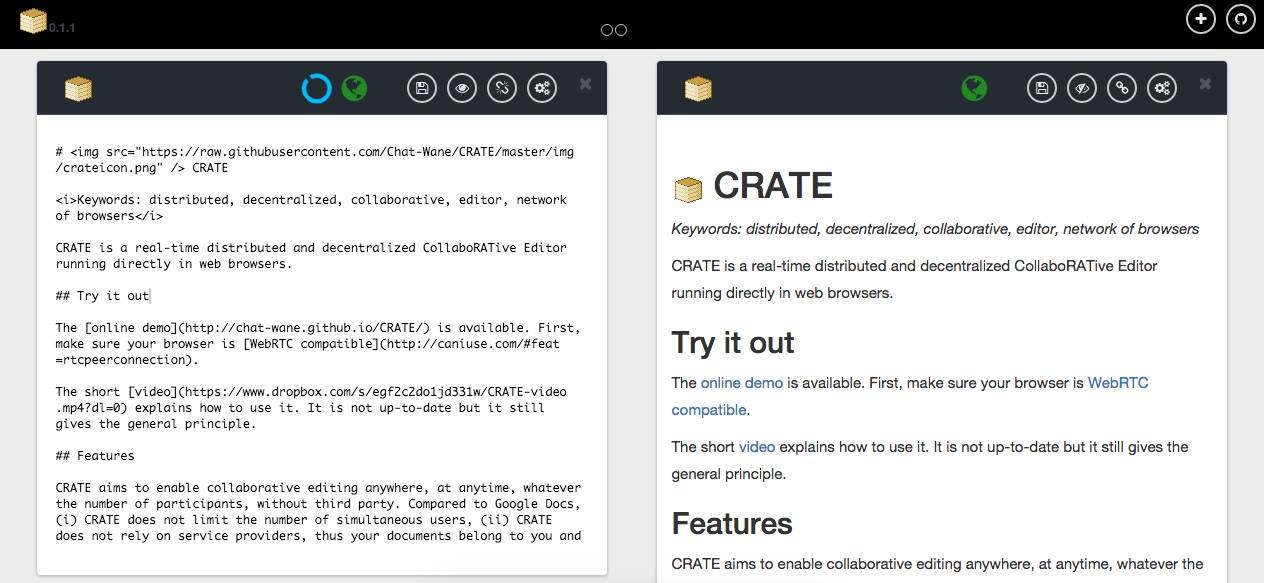
\includegraphics[width=\textwidth]{./img/screenshot.png}
  \caption{\label{img:screenshot} Screenshot of the web application containing
    two editors: on the left, a document is written in markdown language which
    is previewed on the right editor.}
\end{figure*}


%%% Local Variables:
%%% mode: latex
%%% TeX-master: "../paper"
%%% End:
